\begin{frame}[hoved]
	\frametitle{Design}
	\begin{minipage}[t]{0.45\textwidth}
		{\large Requirements}
		\begin{itemize}
			\item Merge sort algorithm capable of running on a bare-metal RISC-V
			      processor.
			\item Capable of running on multiple cores.
			\item Capable of sorting lists of varying sizes.
		\end{itemize}
		{\large Bare-metal}
		\begin{itemize}
			\item Also known as Embedded system programming.
			\item Applications running without an underlying operating system.
			\item A lot of standard library implementations do not work out of the
			      box.
		\end{itemize}
	\end{minipage}
	\hfill
	\begin{minipage}[t]{0.45\textwidth}
		\begin{figure}
			\begin{center}
				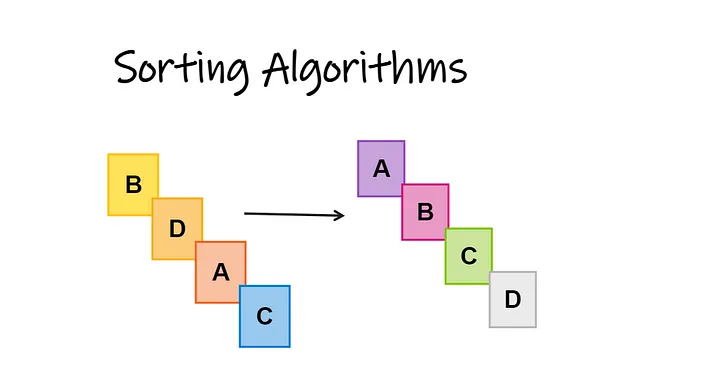
\includegraphics[width=0.95\textwidth]{figures/sorting.png}
			\end{center}
			\caption{\tiny https://medium.com/@noransaber685/understanding-sorting-algorithms-5575d52f5a18}\label{fig:}
		\end{figure}
	\end{minipage}
\end{frame}


\begin{frame}[hoved]
	\frametitle{Design}
	{\large Bare-metal continued}
	\begin{itemize}
		\item Processor uses RISC-V ISA with extensions:
		\item Control and Status Register(Zicsr). (mhartid)
		\item Atomic Instructions(a). (amoadd.w)
		\item Integer Multiplication and Division (m).
		\item Compressed Instructions (c). (bnez, lw). Mainly used for code size
		      reduction.
	\end{itemize}
\end{frame}


\begin{frame}[hoved]
	\frametitle{Design}
	\begin{minipage}[t]{0.45\textwidth}
		{\large Memory continued}
		\begin{itemize}
			\item Use context switching.
			\item Separate core memory and thread memory.
			\item When I had issues with corrupted data, I would thus know have an
			      idea where it was happening.
		\end{itemize}
	\end{minipage}
	\hfill
	\begin{minipage}[t]{0.45\textwidth}
		\begin{figure}
			\begin{center}
				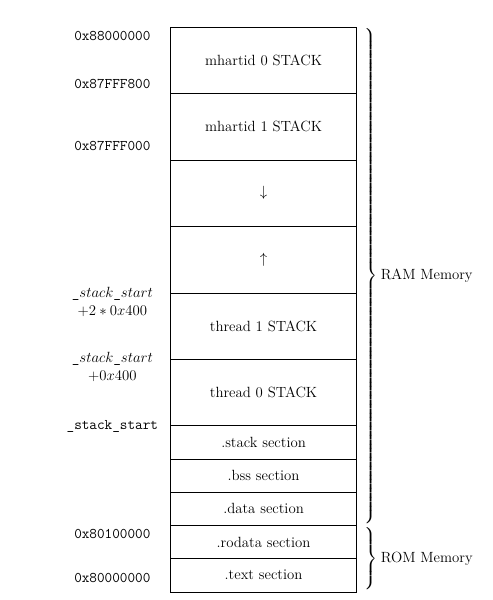
\includegraphics[height=0.65\textheight]{figures/memory.png}
			\end{center}
			\caption{Design of memory layout.}\label{fig:mem_layout}
		\end{figure}
	\end{minipage}
\end{frame}
